\section{Feb 09 Review Questions}
\begin{QandA}
   \item What are differences between strong leases and weak leases and the guarantees they provide?
         \begin{answered}
		 One difference between strong leases and weak leases is that strong leases do not allow the write while the lease held by the cache
		 hasn't expired or the leaseholder hasn't approved the write. If one object is covered by multiple strong leases, the write can happen
		 if all the leaseholders approve the write or all the leases covered that object has expired. This mechanism guarantees that there
		 will be no conflict of write to the object in cache. However, that's not ture for the weak lease. Weak leases allow the writes and reads
		 simultaneously. Same object can be owned by several weak leases with different expiration time. This implies that some leases
		 that are expired allow the writes while other non-expired leases allow the read only. Thus, we may get the conflict on the object in cache.
		 In the write-back cache, the conflict is resolved on the server side. In addition, for the weak leases,
		 the server doesn't need to keep track of the leases granted but that's not true for strong leases. Lastly, strong leases guarantess a strict
		 consistency while the weak leases have a weak consistency. As the consequence, weak lease has better performance than the strong lease
		 as we don't need to queue the writes say in the write-through for the weak lease.
         \end{answered}

   \item Use the types of anomalies allowed to per-object sequential consistency and read-after-write consistency to compare the two consistency models. Is one stronger? If so, which one?
         \begin{answered}
		 For anomalies in vetrices, both per-object sequential consistency and read-after-write consistency have stale read anomalies.
		 In addition, read-after-write consistency also has total order anomalies whereas the per-object sequential consistency doesn't. 
		 If we take a look at the actual statistics, per-object sequential consistency contains 607 total anomalise including 378 stale read
		 anomalies and 229 total order anomalies. Read-after-write consistency contains only total order anomalies. Since there is overlap between
		 read-after-write consistency anomalies and per-object sequential consistency anomalies but one of them is not the subset of the other.
		 Thus, we cannot determine which consistency model is stronger. The above text is illustrated in the Figure \ref{0209-02} as well.
		 \begin{figure}
		 \centering
		 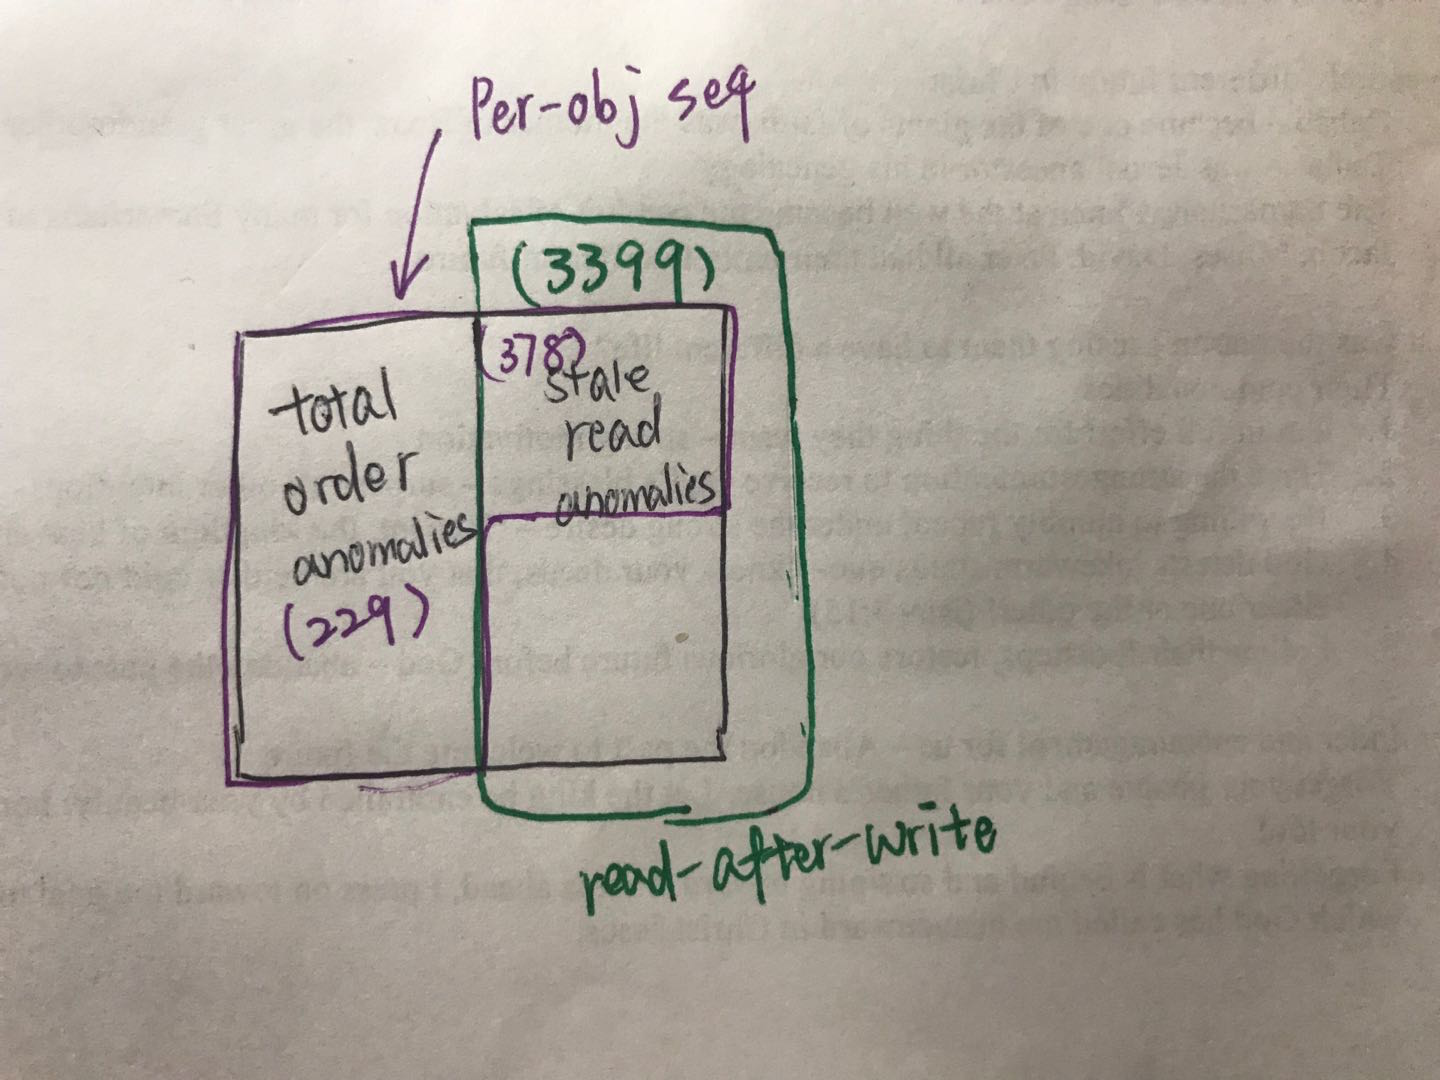
\includegraphics[width=5cm, height=4cm]{0209-02.jpeg} 
		 \caption{Illustration of statistic relationship between two consistency models}
		 \label{0209-02}
		 \end{figure}
         \end{answered}
         
   \item What performance vs consistency tradeoffs are made by Yahoo's different read types (read-any, read-critical, and read-latest)?
         \begin{answered}
    	 \texttt{Read-any} emphasizes performance over consistency.Since the latest read doesn't need to reflect the latest write (i.e.,
    	 we can still read the stale version of the record even after a sucessful write), we can maximize our performance by return a valid
    	 version of record from the records' history. However, for \texttt{Read-critical} and \texttt{Read-latest}, we emphasize the consistency
    	 over the performance. \texttt{Read-critical} requires the returned version has to be strictly newer or the same as the specified version
    	 and \texttt{Read-latest} requires the return has to be the latest copy of the record that reflects all the previous successful writes.
    	 These two types of reads require the squential consistency for the record and at the same time, if the local cahced copy becomes stale,
    	 we need to fetch a new copy from remote replica, which implies that the performance of these two APIs will be lower than \texttt{Read-any}'s. In addition, since \texttt{Read-critical} can return any version of the record as long as the requirement is met, there
    	 are a fraction of record history that satisfy the constraint and any one of them can work. However, \texttt{Read-latest} can only return
    	 the latest one. Thus, \texttt{Read-latest} has the strongest consistency among the tree with the worst performance.
         \end{answered}
\end{QandA}